\chapter{Progettazione} %------------------------------ CHAPTER TITLE
\thispagestyle{empty}

\newpage
\section{Architettura}
L'architettura ad alto livello che si vuole utilizzare è molto semplice. Essa prevede l'implementazione di un componente SAPI~5 e lo sviluppo di un canale di comunicazione con un engine TTS.
Per facilitare lo svolgimento del progetto si è scelto di utilizzare, in congiunta con il committente, un esempio guida chiamato SALB.
Il progetto SALB implementa l'interfaccia SAPI~5 e al suo interno esegue delle chiamate ad un engine TTS.
Partendo da questo esempio andranno sostituite le varie parti che dovranno subire delle modifiche per poi proseguire fino ad ottenere il prodotto desiderato.
Riassumendo, i vari componenti che verranno utilizzati sono:
\begin{description}
	\item[Interfaccia SAPI~5] interfaccia messa a disposizione dal sistema operativo Microsoft Windows che permette di implementare le funzionalità di sintesi e riconoscimento vocale;
	\item[Implementazione interfaccia SAPI~5] seguendo la specifica SAPI~5 si andranno ad implementare le varie funzionalità di sintesi vocale che potranno essere messe a disposizione attraverso l'interfaccia. L'implementazione fornita dipenderà da un engine TTS.
	\item[Engine TTS] engine di sintesi vocale messo a disposizione dall'azienda. Gli engine di sintesi vocale saranno MaryTTS e Speect.
\end{description}
\newpage

\section{Descrizione dei componenti}
	\subsection{Interfaccia SAPI~5}
	  \begin{figure}[H]
	  	\centering
	  	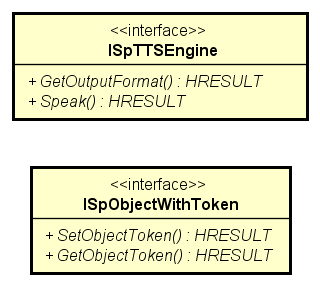
\includegraphics{images/sapi5-interface.png}
	  	\caption{Interfaccia SAPI~5}
	  \end{figure}
 
L'interfaccia SAPI~5 è stata progettata per facilitare il lavoro agli sviluppatori di applicazioni e di engine TTS. Il suo scopo è quello di standardizzare il modo con cui avviene la comunicazione tra applicazioni ed engine TTS. Uno dei task che viene semplificato, utilizzando questa interfaccia, è la gestione del flusso audio. Questo permette agli sviluppatori focalizzarsi maggiormente nello sviluppo dell'engine e non di come il suo output audio venga gestito.
Le interfacce che verranno utilizzate sono ISpTTSEngine e ISpObjectWithToken.
     \subsubsection{ISpObjectWithToken}
     L'interfaccia ISpObjectWithToken permette di creare e reperire le informazioni associate ad un oggetto. Nella maggior parte dei casi l'oggetto viene associato ad una voce.
     \\\\
     \textbf{Metodi}
     \begin{itemize}
     	\item \texttt{+ SetObjectToken(): HRESULT} imposta le proprietà dell'oggetto passato come parametro.
     	\\\\
     	\textbf{Argomenti}
		\begin{itemize}
			\item \texttt{pToken: ISpObjectToken} puntatore all'oggetto che deve essere impostato.
		\end{itemize}
     	\textbf{Valori di ritorno}
		\begin{itemize}
		 	\item \texttt{S\_OK} se la funzione non ha generato errori;
		 	\item \texttt{E\_POINTER} se il parametro \texttt{pToken} non è valido o è malformato;
		 	\item \texttt{E\_OUTOFMEMORY} se la memoria disponibile non è sufficiente;
		 	\item \texttt{FAILED(hr)} se c'è un errore da ritornare. 
		 \end{itemize}
	    
	     \item \texttt{+ GetObjectToken(): HRESULT} serve per ottenere un oggetto settato in precedenza. L'oggetto verrà restituito come parametro.
	     \\\\
	     \textbf{Argomenti}
		 \begin{itemize}
		     \item \texttt{ppToken: ISpObjectToken} indirizzo dell'oggetto richiesto.
		 \end{itemize}
	     \textbf{Valori di ritorno}
		 \begin{itemize}
		    \item \texttt{S\_OK} se la funzione non ha generato errori;
		    \item \texttt{E\_POINTER} se il parametro \texttt{ppToken} non è valido o è malformato;
		    \item \texttt{E\_OUTOFMEMORY} se la memoria disponibile non è sufficiente;
	     	\item \texttt{FAILED(hr)} se c'è un errore da ritornare. 
	     \end{itemize}
     \end{itemize}
      
     \subsubsection{ISpTTSEngine}
     ISpTTSEngine è l'interfaccia principale della specifica SAPI~5. Essa svolge i due compiti principali della sintesi vocale che sono le chiamate all'engine TTS e la generazione dell'audio in un formato specifico. Inoltre gestisce anche gli eventi generati dalla sintesi vocale.
     \\\\
     \textbf{Metodi}
     \begin{itemize}
     	\item \texttt{+ GetOutputFormat(): HRESULT} ritorna il formato audio previsto dall'engine TTS;
     	\\\\
		\textbf{Argomenti}
		\begin{itemize}
			\item \texttt{pTargetFmtId: GUID} id del formato richiesto come uscita. I valori possibili possono essere di due tipi: \texttt{SPDFID\_Text} per ottenere un formato testuale e \texttt{SPDFID\_WAVEFORMATEX} per un formato audio;
			\item \texttt{pTargetWaveFormatEx: WAVEFORMATEX} se l'identificatore del formato è del tipo \texttt{SPDFID\_WAVEFORMATEX} l'argomento contiene il puntatore alla struttura del formato audio, altrimenti il suo valore è \texttt{NULL};
			\item \texttt{pOutputFormatId: GUID} contiene l'identificatore del formato di uscita che può essere \texttt{SPDFID\_Text} o \texttt{SPDFID\_WAVEFORMATEX}
			\item \texttt{ppCoMemOutputWaveFormatEx: WAVEFORMATEX} contiene la struttura di tipo \texttt{WAVEFORMATEX} del formato audio se l'argomento \texttt{pOutputFormatId} è impostato al valore \texttt{SPDFID\_WAVEFORMATEX} altrimenti è \texttt{NULL}. La struttura verrà allocata tramite \texttt{CoTaskMemAlloc}.
		\end{itemize}
		\item \texttt{+ Speak(): HRESULT} è il metodo che effettua la sintesi vocale trasformando l'input testuale in un formato specifico.
		\\\\
		\textbf{Argomenti}
		\begin{itemize}
			\item \texttt{dwSpeakFlags: DWORD} contiene i valori dei flags che descrivono le caratteristiche dell'input;
			\item \texttt{rguidFormatId: GUID} identificatore del formato di uscita della sintesi vocale. I possibili valori possono essere \texttt{SPDFID\_Text} o \texttt{SPDFID\_WAVEFORMATEX};
			\item \texttt{pWaveFormatEx: WAVEFORMATEX} puntatore alla struttura che descrive il formato d'uscita se il parametro \texttt{rguidFormatId} ha valore \texttt{SPDFID\_WAVEFORMATEX}. L'argomento ha valore \texttt{NULL} se il parametro \texttt{rguidFormatId} ha valore \texttt{SPDFID\_Text};
			\item \texttt{pTextFragList: SPVTEXTFRAG} lista concatenata di \texttt{SPVTEXTFRAG} su cui eseguire la sintesi vocale. Un elemento \texttt{SPVTEXTFRAG} è formato da un frammento di testo decorato da altri atttributi che ne descrivono meglio le caratteristiche;
			\item \texttt{pOutputSite: ISpTTSEngineSite} è il puntatore all'interfaccia \texttt{ISpTTSEngineSite} che viene utilizzato per scrivere l'audio e aggiungere gli eventi SAPI alla coda gestita dall'interfaccia.
		\end{itemize}  
	\end{itemize}

	\subsubsection{Descrizione del funzionamento}
	Per comprendere al meglio il funzionamento dell'interfaccia SAPI~5 verranno descritte le operazioni che tipicamente vengono eseguite.
	Per prima cosa viene effettuata l'inizializzazione dell'engine TTS tramite il metodo \texttt{ISpObjectWithToken::SetObjectToken()}. Questo permette di ottenere un oggetto che può essere utilizzato dall'engine per eseguire la sua inizializzazione.
	Ad esempio attraverso questa operazione è possibile impostare la voce con cui verrà effettuata la sintesi vocale.
	Una volta che l'engine è stato inizializzato è possibile recuperare le sue informazioni tramite il metodo \texttt{ISpObjectWithToken::GetObjectToken()} e di renderle disponibili, se richieste, ad applicazioni o altri componenti.
	Il compito principale di sintesi vocale è affidato al metodo \texttt{ISpTTSEngineSite::Speak()} che si occupa di ricevere l'input testuale, somministrarlo all'engine TTS e scrivere l'output audio in buffer che verrà riprodotto dall'sistema operativo.
	Il formato audio che si vuole scrivere deve essere specificato tramite il metodo \texttt{ISpTTSEngineSite::GetOutputFormat()} in modo che l'acquisizione e la riproduzione avvenga nel modo corretto.\\\\
	\textbf{Eventi}\\
	L'interfaccia SAPI~5 è stata progettata ad eventi e questo comporta che ogni cambiamento di stato sia determinato da un evento.\\
	Un evento SAPI è definito da una struttura chiamata \texttt{SPEVENT} che è composta da i seguenti attributi:
	\begin{itemize}
		\item \texttt{eEventId: WORD} identifica il tipo di evento tramite un enumeratore;
		\item \texttt{elParamType: WORD} definisce tramite un enumeratore il tipo di \texttt{lParam};
		\item \texttt{ulStreamNum: ULONG} identifica a quale stream appartiene l'evento. Nel nostro caso l'engine TTS non deve preoccuparsi di settare questo parametro, perchè sarà compito dell'applicazione;
		\item \texttt{ullAudioOffset: ULONGLONG} rappresenta l'offset dello stream audio espresso in termini di byte. Buona norma è che questo valore coincida con l'inizio di un campione audio;
		\item \texttt{wParam: WPARAM} è un campo generico che può contenere le informazioni associate all'evento;
		\item \texttt{lParam: LPARAM} è un campo generico che può contenere le informazioni associate all'evento.
	\end{itemize}
	Adesso andremo ad analizzare gli eventi che possono essere gestiti dall'interfaccia SAPI in base al loro \texttt{eEventId}: 
	\begin{description}
		\item [] \texttt{SPEI\_TTS\_BOOKMARK} è l'evento associato al raggiungimento di un \texttt{BOOKMARK}.\\
		I suoi campi generici assumono i seguenti significati:
		\begin{itemize}
			\item \texttt{wParam} contiene la conversione della stringa associata al \texttt{BOOKMARK} nel valore numerico;
			\item \texttt{lParam} contiene la stringa associata al \texttt{BOOKMARK}.
		\end{itemize}
		\item [] \texttt{SPEI\_WORD\_BOUNDARY} è l'evento sollevato in corrispondenza dell'inizio di una parola. Esso viene spesso utilizzato per ottenere l'evidenziazione di una parola sintetizzata in un testo.\\
		I suoi campi generici assumono i seguenti significati:
		\begin{itemize}
			\item \texttt{wParam} rappresenta l'offset espresso in caratteri rispetto all'inizio dell'input;
			\item \texttt{lParam} contiene la lunghezza espressa in caratteri della parola che deve essere sintetizzata.
		\end{itemize}
		\item [] \texttt{SPEI\_SENTENCE\_BOUNDARY} è l'evento sollevato in corrispondenza dell'inizio di una frase.\\
		I suoi campi generici assumono i seguenti significati:
		\begin{itemize}
			\item \texttt{wParam} rappresenta l'offset espresso in caratteri rispetto all'inizio dell'input;
			\item \texttt{lParam} contiene la lunghezza espressa in caratteri della frase che deve essere sintetizzata.
		\end{itemize}
		\item [] \texttt{SPEI\_PHONEME} è l'evento sollevato in corrispondenza della presenza di un fonema. Esso può essere utilizzato per effettuare lo spelling fonetico del testo.\\
		I suoi campi generici assumono i seguenti significati:
		\begin{itemize}
			\item \texttt{wParam} è diviso in due \texttt{WORD}, la \texttt{WORD} più significativa contiene la durata in millisecondi del fonema corrente, invece la \texttt{WORD} meno significativa contiene il \texttt{PhoneID} del fonema successivo;
			\item \texttt{lParam} è diviso in due \texttt{WORD}, la \texttt{WORD} più significativa contiene la \texttt{SPVFEATURE} associata al fonema, invece la \texttt{WORD} meno significativa contiene il \texttt{PhoneID} del fonema corrente.
		\end{itemize}
		\item [] \texttt{SPEI\_VISEME} è l'evento sollevato in corrispondenza della presenza di un visema. Gli eventi di questo tipo possono essere utilizzati per pilotare un avatar.\\
		I suoi campi generici assumono i seguenti significati:
		\begin{itemize}
			\item \texttt{wParam} è diviso in due \texttt{WORD}, la \texttt{WORD} più significativa contiene la durata in millisecondi del visema corrente, invece la \texttt{WORD} meno significativa contiene l'identificatore del visema successivo;
			\item \texttt{lParam} è diviso in due \texttt{WORD}, la \texttt{WORD} più significativa contiene la \texttt{SPVFEATURE} associata al visema, invece la \texttt{WORD} meno significativa contiene l'identificatore del visema corrente.
		\end{itemize}
	\end{description}
	L'interfaccia SAPI affida la gestione degli eventi ad una coda. Durante la chiamata al metodo \texttt{ISpTTSEngine::Speak()} è possibile eseguire l'inserimento degli eventi nella coda tramite il metodo \texttt{ISpTTSEngineSite::AddEvents()} mediante l'argomento \texttt{pOutputSite}.
	L'aspetto più importante è dato dalla relazione che esiste tra lo stream audio e gli eventi. Infatti le due entità vengono trattate come se lo stream audio fosse la linea del tempo e gli eventi degli avvenimenti che accadono in determinato momento identificato dal campo \texttt{ullAudioOffset}.
	%immagine linea del tempo con eventi
	\\\\
	\textbf{Azioni}\\
	Lo standard SAPI~5 permette la gestione di azioni che avvengono in tempo reale. Ad esempio è possibile controllare il volume dell'uscita audio o la sua velocità.
	Per fare ciò bisogna utilizzare il metodo \texttt{ISpTTSEngineSite::GetActions()} messo a disposizione dall'argomento \texttt{pOutputSite}.
	L'invocazione del metodo permette di capire quali azioni sono state effettuate dall'applicazione.Esse possono essere di tre tipi:
	\begin{itemize}
		\item \texttt{SPVES\_VOLUME} se il volume è stato cambiato;
		\item \texttt{SPVES\_RATE} se la velocità è stata cambiata;
		\item \texttt{SPVES\_SKIP} se è stata espressa l'intenzione di spostarsi ad un certo punto del testo;
		\item \texttt{SPVES\_ABORT} se la sintesi è stata interrotta;
		\item \texttt{SPVES\_CONTINUE} se nessuna delle precedenti azioni è stata eseguita;
	\end{itemize}
	Nei i primi tre casi l'interfaccia SAPI mette a disposizione dei metodi per recuperare i nuovi valori e sono rispettivamente:
	\begin{itemize}
		\item \texttt{ISpTTSEngineSite::GetVolume(): HRESULT} per recuperare il nuovo valore del volume;
		\item \texttt{ISpTTSEngineSite::GetRate(): HRESULT} per recuperare il nuovo valore della velocità;
		\item \texttt{ISpTTSEngineSite::GetSkipInfo(): HRESULT} per recuperare il tipo e il numero di unità da saltare in avanti o indietro rispetto al punto in cui la sintesi è arrivata. Per completare l'operazione c'è il bisogno di invocare il metodo \texttt{ISpTTSEngineSite::CompleteSkip()} che verifica se è possibile portare a termine l'azione;
	\end{itemize}	
	Un altro parametro della voce su cui è possibile agire è la tonalità. In questo caso la regolazione non avviene come per la velocità o il volume, ma si deve agire sulla proprietà \texttt{PitchAdj} associata agli elementi della lista \texttt{pTextFragList}.
	